\documentclass[11pt,a4paper]{article}

% ======== PAQUETES BÁSICOS ========
\usepackage[utf8]{inputenc}    % Acentos
\usepackage[T1]{fontenc}
\usepackage[spanish]{babel}    % Idioma español
\usepackage{amsmath, amssymb, amsfonts}  % Matemática
\usepackage{graphicx}          % Imágenes
\usepackage{physics}           % Derivadas, gradientes, etc.
\usepackage{siunitx}           % Unidades físicas (m, s, kg, etc.)
\usepackage{xcolor}            % Colores
\usepackage{geometry}          % Márgenes
\usepackage{fancyhdr}          % Encabezado/pie
\usepackage{hyperref}          % Enlaces
\usepackage{listings}          % Código fuente
\usepackage{caption}           % Subtítulos en código
\usepackage{tcolorbox}         % Cajas para resúmenes o ejemplos

% ======== CONFIGURACIÓN DE PÁGINA ========
\geometry{margin=2cm}
\pagestyle{fancy}
\fancyhf{}
\rhead{Apuntes de Física y Python}
\lhead{Israel Bravo — UdeC}
\cfoot{\thepage}

% ======== CONFIGURACIÓN DE CÓDIGO PYTHON ========
\definecolor{lightgray}{gray}{0.95}
\definecolor{darkgreen}{rgb}{0,0.5,0}
\lstset{
    language=Python,
    backgroundcolor=\color{lightgray},
    commentstyle=\color{darkgreen},
    keywordstyle=\color{blue}\bfseries,
    stringstyle=\color{red},
    basicstyle=\ttfamily\footnotesize,
    frame=single,
    numbers=left,
    numberstyle=\tiny\color{gray},
    breaklines=true,
    showstringspaces=false,
    tabsize=4
}

% ======== ESTILO DE CAJAS ========
\tcbset{
    colback=blue!5!white,
    colframe=blue!70!black,
    fonttitle=\bfseries,
    coltitle=black,
    boxrule=0.8pt,
    arc=3pt
}

% ======== INICIO DEL DOCUMENTO ========
\begin{document}

\begin{center}
    {\LARGE \textbf{Derivadas numericas y derivadas Discretas}}\\[4pt]
    {\large Universidad de Concepción — Israel Bravo}\\[10pt]
    \hrulefill
\end{center}

\section{Derivadas analiticas y numericas}
Empezaremos estudiando como calcular derivadas numericas sabiendo la definicion analitica
que tiene esta funcion. Probemos derivando La funcion $sen(x)$, Todos sabemos que la derivada
del seno es coseno, por lo tanto podemos plantear lo siguiente:

\begin{lstlisting}[caption=Derivar seno numericamente]
import numpy as np
import matplotlib.pyplot as plt

h = 0.01
x = np.linspace(-2*np.pi,2*np.pi,30)
df = (np.sin(x+h)-np.sin(x))/(h)
f = np.sin(x)
derivadaanalitica = np.cos(x)

plt.plot(x,df,color='blue',label = 'Derivada numerica')
plt.plot(x,derivadaanalitica,color = 'red',linestyle='--',label = 'Derivada analitica')
plt.grid(True)
plt.xlabel('x')
plt.ylabel('y')
plt.legend()
plt.show()

\end{lstlisting}
Dandonos los siguientes graficos:

\begin{figure}[h!]
    \centering
    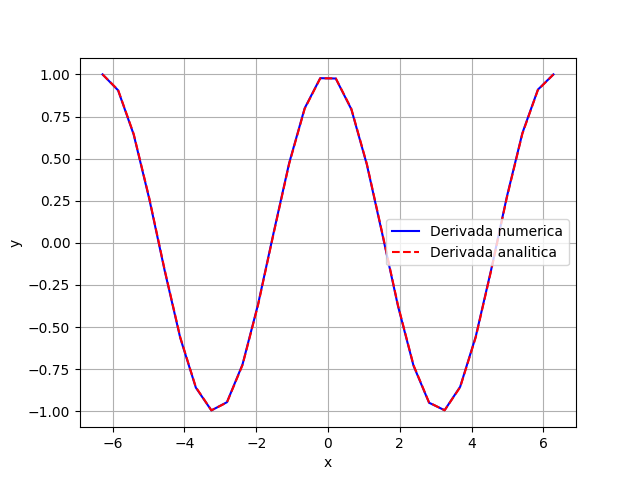
\includegraphics[width=0.45\textwidth]{img/derivadascomparadas.png}
    \hfill % Espacio horizontal entre las imágenes
    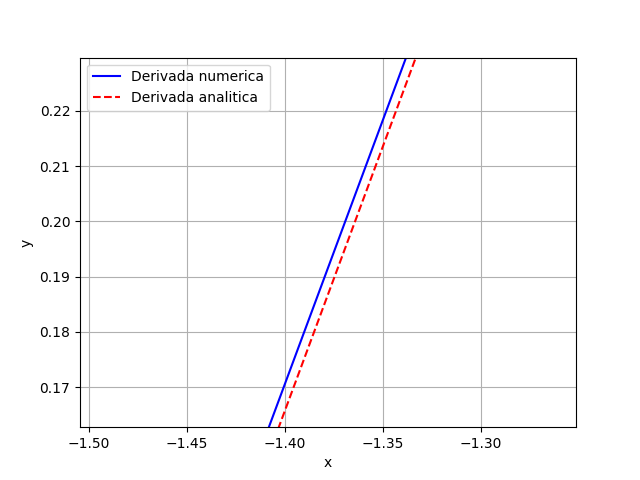
\includegraphics[width=0.45\textwidth]{img/derivadascomparadaserror.png}
    \caption{Comparación de las derivadas y como cambian dependiendo del h. La figura de la izquierda muestra la comparación de las derivadas, mientras que la de la derecha muestra como se ven desde muy cerca.}
    \label{fig:derivadas_comparadas}
\end{figure}

Existen muchos tipos de derivadas, pero todas salen del mismo lugar, Basicamente son deducciones
de jugar con el Teorema de Taylor. por ejemplo, esta derivada que calculamos es una derivada
adelantada.
\bigskip
Por teorema de Taylor tenemos:
\begin{equation}
 f(x+h) = f(x) + hf'(x) + \frac{h^2}{2!}f''(x) + \frac{h^3}{3!}f'''(x) + \dots + \frac{h^n}{n!}f^{(n)}(x) + \dots
\end{equation}
Si despejamos $f'$ nos quedaria lo siguiente:

\begin{equation}
    f'(x) = \frac{f(x+h) - f(x)}{h} - \left( \frac{h}{2!}f''(x) + \frac{h^2}{3!}f'''(x) + \dots \right)
\end{equation}



\end{document}

